%这个是根据计算机学报官网下的LaTeX模板改的,主要修改内容:①把GBK编码改成了UTF-8编码。②引入zhwinfonts,用上传的字体文件实现了字体的使用。
%现存的问题:①中文无法使用加粗功能,但是英文可以。解决方式1:使用黑体来凑合代替。解决方式2:在PDF编辑器里面一个一个加粗。②无法实现模板中所要求的每页脚注从1开始的要求。
%如果您在使用该模板的过程中遇到问题,或者有对该模板的修改意见,请联系本人:微信PolarisRisingWar(诸神缄默不语),或者CSDN诸神缄默不语(PolarisRisingWar)

\documentclass[10.5pt,compsoc]{CjC}
\usepackage{CJKutf8}
%\usepackage{CJK}
\usepackage{graphicx}
\usepackage{footmisc}
\usepackage{subfigure}
\usepackage{url}
\usepackage{multirow}
\usepackage[noadjust]{cite}
\usepackage{amsmath,amsthm}
\usepackage{amssymb,amsfonts}
\usepackage{booktabs}
\usepackage{color}
\usepackage{ccaption}
\usepackage{booktabs}
\usepackage{float}
\usepackage{fancyhdr}
\usepackage{caption}
\usepackage{xcolor,stfloats}
\usepackage{comment}
\setcounter{page}{1}
\graphicspath{{figures/}}
\usepackage{cuted}%flushend,
\usepackage{captionhack}
\usepackage{epstopdf}
\usepackage[utf8]{inputenc}
\definecolor{codebackground}{rgb}{0.95,0.95,0.95}
\definecolor{codekeyword}{rgb}{0.08,0.39,0.63}
\definecolor{codestring}{rgb}{0.7,0.1,0.1}
\definecolor{codecomment}{rgb}{0.46,0.64,0.46}

%\usepackage{ccmap}
%\CJKtilde
%\usepackage{CJKpunct} 
%\usepackage[lite,subscriptcorrection,slantedGreek,nofontinfo]{mtpro2}

%===============================%

%\firstfootname{ \quad \quad }
\headevenname{\mbox{\quad} \hfill  \mbox{\zihao{-5}{\begin{CJK*}{UTF8}{song}计\quad \quad 算\quad \quad 机\quad \quad 学\quad \quad 报\end{CJK*}} \hspace {50mm} \mbox{\begin{CJK*}{UTF8}{song}2019 年\end{CJK*}}}}%
\headoddname{\begin{CJK*}{UTF8}{song}? 期 \hfill
作者姓名等:论文题目\end{CJK*}}%

%footnote use of *
\renewcommand{\thefootnote}{\fnsymbol{footnote}}
\setcounter{footnote}{0}
\renewcommand\footnotelayout{\zihao{5-}}

\newtheoremstyle{mystyle}{0pt}{0pt}{\normalfont}{1em}{\bf}{}{1em}{}
\theoremstyle{mystyle}
\renewcommand\figurename{figure~}
\renewcommand{\thesubfigure}{(\alph{subfigure})}
\newcommand{\upcite}[1]{\textsuperscript{\cite{#1}}}
\renewcommand{\labelenumi}{(\arabic{enumi})}
\newcommand{\tabincell}[2]{\begin{tabular}{@{}#1@{}}#2\end{tabular}}
\newcommand{\abc}{\color{white}\vrule width 2pt}
\makeatletter
\renewcommand{\@biblabel}[1]{[#1]\hfill}
\makeatother
\setlength\parindent{2em}
%\renewcommand{\hth}{\begin{CJK*}{UTF8}{zhhei}}
%\renewcommand{\htss}{\begin{CJK*}{UTF8}{song}}

\input{zhwinfonts}
\begin{document}
\hyphenpenalty=50000
\makeatletter
\newcommand\mysmall{\@setfontsize\mysmall{7}{9.5}}
\newenvironment{tablehere}
  {\def\@captype{table}}

\let\temp\footnote
\renewcommand \footnote[1]{\temp{\zihao{-5}#1}}


\thispagestyle{plain}%
\thispagestyle{empty}%
\pagestyle{CjCheadings}

\begin{table*}[!t]
\vspace {-13mm}
\begin{tabular}{p{168mm}}
\zihao{5-}\begin{CJK*}{UTF8}{song}
第??卷\quad 第?期 \hfill 计\quad 算\quad 机\quad 学\quad 报\hfill Vol. ??  No. ?\end{CJK*}\\
\zihao{5-}\begin{CJK*}{UTF8}{song}
20??年?月 \hfill CHINESE JOURNAL OF COMPUTERS \hfill ???. 20??\end{CJK*}\\
\hline\\[-4.5mm]
\hline\end{tabular}

\centering
\vspace {11mm}
\begin{CJK*}{UTF8}{zhhei}
{\zihao{2} 题目(中英文题目一致)字体为2号黑体(全文除特别声明外, 外文统一用Times New Roman) }
\end{CJK*}
\vskip 5mm

{\zihao{3}\begin{CJK*}{UTF8}{fs}
作者名$^{1)}$\quad  作者名$^{2),3)}$ \quad 作者名$^{3) }$($^*$字体为3号仿宋*作者)\end{CJK*}}

\vspace {5mm}
\zihao{6}{\begin{CJK*}{UTF8}{song}
$^{1)}$(单位全名 部门(系)全名, 市(或直辖市) 国家名 邮政编码)
*字体为6号宋体*单位
\end{CJK*}}

\zihao{6}{\begin{CJK*}{UTF8}{song}
$^{2)}$(单位全名 部门(系)全名, 市(或直辖市) 国家名
邮政编码)*中英文单位名称、作者姓名须一致*
\end{CJK*}}

\zihao{6}{\begin{CJK*}{UTF8}{song}
$^{3)}$(单位全名 部门(系)全名, 市(或直辖市) 国家名 邮政编码)
\end{CJK*}}

\zihao{6}{\begin{CJK*}{UTF8}{zhhei}
论文定稿后,作者署名、单位无特殊情况不能变更。若变更,须提交签章申请,国家名为中国可以不写,省会城市不写省的名称,其他国家必须写国家名。
\end{CJK*}}

\vskip 5mm
{\centering
\begin{tabular}{p{160mm}}
\zihao{5-}{
\setlength{\baselineskip}{16pt}\selectfont{
\noindent\begin{CJK*}{UTF8}{zhhei}摘\quad 要\quad \end{CJK*} \begin{CJK*}{UTF8}{song}
*中文摘要内容置于此处(英文摘要中要有这些内容),字体为小5号宋体。摘要贡献部分,要有数据支持,不要出现``...大大提高''、``...显著改善''等描述,正确的描述是``比{\ldots}提高X{\%}''、
``在{\ldots}上改善X{\%}''。*摘要

\end{CJK*}\par}}\\[2mm]

\zihao{5-}{\noindent
\begin{CJK*}{UTF8}{zhhei}关键词\end{CJK*} \quad \begin{CJK*}{UTF8}{song}{*关键词(中文关键字与英文关键字对应且一致,应有5-7个关键词);关键词;关键词;关键词*  }
\end{CJK*}
}\\[2mm]
\zihao{5-}{\begin{CJK*}{UTF8}{zhhei}中图法分类号\end{CJK*}	\begin{CJK*}{UTF8}{song}
TP\end{CJK*}\rm{\quad \quad \quad     }
\begin{CJK*}{UTF8}{zhhei}DOI号:\end{CJK*}\begin{CJK*}{UTF8}{song}
*投稿时不提供DOI号\end{CJK*}}
\end{tabular}}

\vskip 7mm

\begin{center}
\zihao{3}{ {\begin{CJK*}{UTF8}{zhhei}Title *(中英文题目一致)字体为4号Times New Roman,加粗* Title\end{CJK*}}}\\
\vspace {5mm}
\zihao{5}{ {\begin{CJK*}{UTF8}{zhhei}NAME Name-Name$^{1)}$ NAME Name$^{2)}$ NAME Name-Name$^{3)}$ *字体为5号Times
new Roman*Name\end{CJK*}
}}\\
\vspace {2mm}
\zihao{6}{\begin{CJK*}{UTF8}{zhhei}{$^{1)}$(Department of ****, University, City ZipCode, China) *字体为6号Times
new Roman* Depart.Correspond}\end{CJK*}}

\zihao{6}{\begin{CJK*}{UTF8}{zhhei}{$^{2)}$(Department of ****, University, City ZipCode)*中国不写国家名*}\end{CJK*}}

\zihao{6}{\begin{CJK*}{UTF8}{zhhei}{$^{3)}$(Department of ****, University, City ZipCode, country)*外国写国家名*}\end{CJK*}}



\end{center}

\begin{tabular}{p{160mm}}
\zihao{5}{
\setlength{\baselineskip}{18pt}\selectfont{
{\bf Abstract}\quad \begin{CJK*}{UTF8}{zhhei}(\textbf{500英文单词,内容包含中文摘要的内容}).
字体为Times new Roman,字号5号* Abstract\end{CJK*}
\par}}\\

\setlength{\baselineskip}{18pt}\selectfont{
\zihao{5}{\noindent Do not modify the amount of space before and after the artworks. One- or two-column format artworks are preferred. and Tables, create a new break line and paste the resized artworks where desired. Do not modify the amount of space before and after the artworks. One- or two-column format artworks are preferred. All Schemes, Equations, Figures, and Tables should be mentioned in the text consecutively and numbered with Arabic numerals, and appear below where they are mentioned for the first time in the main text. To insert Schemes, Equations, Figures, and Tables, create a new break line and paste the resized artworks where desired. Do not modify the amount of space before and after the artworks. One- or two-column format artworks are preferred.Do not modify the amount of space before and after the artworks. One- or two-column format artworks are preferred. and Tables, create a new break line and paste the resized artworks where desired. Do not modify the amount of space before and after the artworks. One- or two-column format artworks are preferred. All Schemes, Equations, Figures, and Tables should be mentioned in the text consecutively and numbered with Arabic numerals, and appear below where they are mentioned for the first time in the main text.

\vspace {5mm}
{\bf Keywords}\quad \begin{CJK*}{UTF8}{zhhei}中文关键字与英文关键字对应且一致,\textbf{不要用英文缩写});
key word; key word; key word* *字体为5号Times new Roman * Key words\end{CJK*}}\par}
\end{tabular}

\setlength{\tabcolsep}{2pt}
\begin{tabular}{p{0.05cm}p{16.15cm}}
\multicolumn{2}{l}{\rule[4mm]{40mm}{0.1mm}}\\[-3mm]
&\begin{CJK*}{UTF8}{song}
收稿日期:\quad \quad -\quad -\quad ;最终修改稿收到日期:\quad \quad -\quad -\quad .*投稿时不填写此项*. 本课题得到… …基金中文完整名称(No.项目号)、… …基金中文完整名称(No.项目号)、… … 基金中文完整名称(No.项目号)资助.作者名1(通信作者),性别,xxxx年生,学位(或目前学历),职称,是/否计算机学会(CCF)会员(提供会员号),主要研究领域为*****、****.E-mail: **************.作者名2(通信作者),性别,xxxx年生,学位(或目前学历),职称,是/否计算机学会(CCF)会员(提供会员号),主要研究领域为*****、****.E-mail: **************. 作者名3(通信作者),性别,xxxx年生,学位(或目前学历),职称,是/否计算机学会(CCF)会员(提供会员号),主要研究领域为*****、****.E-mail: **************.(给出的电子邮件地址应不会因出国、毕业、更换工作单位等原因而变动。请给出所有作者的电子邮件)
第1作者手机号码(投稿时必须提供,以便紧急联系,发表时会删除): … …, E-mail: … …*此部分6号宋体*
\end{CJK*}
\end{tabular}\end{table*}
\clearpage\clearpage
\begin{strip}
\vspace {-13mm}
\end{strip}
    \linespread{1.15}
    \begin{CJK*}{UTF8}{zhhei}
\zihao{5}
\vskip 1mm
\section{研究背景}
在本项目的研究进程中,本人(何锦诚)主要负责基于大模型 API 开展数据集的批量处理工作,并通过提示词工程对模型在数据集上的表现进行优化提升。代码仓库在https://github.com/JacksonHe04/smart-table-llm。具体工作内容如下:

\section{Zero Shot 相关工作}
首先,本人编写了 Zero-shot 的系统提示词,该提示词的具体内容存储于 zero-shot-prompt.js 文件中。其核心内容为:"You are an accurate table Q\&A assistant. Please carefully analyze the following table and answer the questions accurately. Note: Only output the answers, do not explain the process. \texttt{table\_text}:table content; \texttt{statement}: question. Please give the answer directly." 

% 在代码实现层面,采用如下 JavaScript 代码进行定义:

% \begin{lstlisting}[language=JavaScript]
% const prompt = {
%   get system() {
%     return "You are an accurate table Q&A assistant.";
%   },
%   generateUserPrompt: (tableText, statement) =>
%     `Please carefully analyze the following table and answer the questions accurately. Note: Only output the answers, do not explain the process.\n\nTable Content: ${tableText}\n\nQuestion:${statement}\n\nPlease give the answer directly.`,
% };
% export default prompt;
% \end{lstlisting}

随后,本人与郑宇榕、李凯文基于测试集的同一个随机子集 test\_100.jsonl 分别展开测试工作。将上述提示词应用到 doubao-1-5-pro-256k 模型上,经测试,该模型在该测试集上的准确率(ACC)达到 57\%,此结果为本后续工作奠定了重要基础。

在针对训练集的工作中,为了更好地优化模型性能,本人设计了将模型在批量处理训练集时回答错误的问题及其内容存储到 wrong\_answers.jsonl 文件的机制。

\subsection{基于训练集的错误案例编写规则提示词}
通过对训练集 train\_lower.jsonl 进行多次随机抽取批量测试,从 to\_train\_rules.jsonl 文件中精心选取了 39 个回答错误的案例。针对这些案例的错误原因展开深入分析,在此基础上,为提示词新增了 15 条规则,并将添加规则后的提示词命名为 jincheng-prompt,其在项目文件中的存储路径为 simple-prompt.js。

基于 simple-prompt.js 提示词,在 doubao-1.5-pro-32k 模型上,对 test\_100.jsonl 测试集进行测试,结果显示准确率(ACC)达到 62\%,相较于 Zero-shot 提示词的 57\%,提升了 5 个百分点。进一步将规则从中文转换为英文后,准确率(ACC)提升至 63\%,较中文规则提示词又提高了 1 个百分点。

% 对应的 JavaScript 代码如下:

% \begin{lstlisting}[language=JavaScript]
% const prompt = {
%   rules: [
%     "Only output the final answer, without any explanation",
%     "The answer must be in exactly the same format as required by the question",
%     "If it is a country name, use the full country name instead of the abbreviation",
%     "If the quantity is asked, the count must be accurate",
%     "If the answer is a number, output the number without any units",
%     "If there are multiple possible answers, only output the one that best meets the requirements of the question",
%     "The answer must be based on the data in the table and do not use external knowledge",
%     "If calculations are involved, they must be accurately calculated without estimation",
%     "Keep the case of the answer consistent with what is required by the question",
%     "For dates and times, keep the original format",
%     "If there are null or missing values in the table, exclude these values during calculations",
%     "For the content within quotation marks, the original format must be maintained, including the quotation marks themselves",
%     "Carefully check all cases that meet the criteria when counting",
%     "For sorting and comparison, consider the data in all relevant columns",
%     "If the answer involves specific text content, it must exactly match the original text, including case and punctuation marks",
%   ],
%   get system() {
%     return (
%       "You are an accurate table Q&A assistant.\n" +
%       this.rules.map((rule, index) => `${index + 1}. ${rule}`).join("\n")
%     );
%   },
%   generateUserPrompt: (tableText, statement) =>
%     `Please carefully analyze the following table and answer the questions accurately. Note: Only output the answers, do not explain the process.\n\nTable Content: ${tableText}\n\nQuestion:${statement}\n\nPlease give the answer directly.`,
% };
% export default prompt;
% \end{lstlisting}

此外,本人在测试集上进行了 5 次独立测试,每次随机抽取 100 个案例,经计算,准确率(ACC)的平均值为 61.60\%,测试日志分别存储于 test-1.txt、test-2.txt、test-3.txt、test-4.txt、test-5.txt 文件中。

\subsection{更复杂的规则提示词}
参考谷歌提示工程指南,本人对提示词进行重新深度优化,新增多条规则并详细给出具体执行步骤,优化后的提示词存储于 prompt.js 文件中。然而,在随机测试 100 个案例后发现,模型准确率(ACC)反而下降至 59\%。经分析,提示词复杂化导致准确率下降的原因主要包括以下几个方面:

\begin{itemize}
  \item \textbf{认知负载增加}:更复杂的提示词包含了更多的规则和步骤,这显著增加了模型的认知负载。当模型需要同时处理和遵循多个复杂规则时,其对核心任务(表格问答)的注意力分配受到影响,进而导致性能下降。
  \item \textbf{规则冲突}:随着规则数量的增多,不同规则之间可能产生潜在的冲突或模糊性,使得模型在决策过程中出现犹豫或错误判断。
  \item \textbf{过度约束}:过多的具体执行步骤在一定程度上限制了模型的灵活性,使其无法充分发挥自身在表格理解和问答方面的能力。
  \item \textbf{输出格式干扰}:复杂的提示词可能使模型过度关注输出格式的规范性,而忽视了答案本身的准确性。
\end{itemize}

\section{One Shot 相关工作}
本人从训练集中选取 1 个案例作为 one-shot 的示例,相关代码存储于 one-shot.js 文件中(该提示词不包含规则)。同样在 doubao-1.5-pro-32k 模型上进行 5 次独立测试,每次随机抽取 100 个案例,经计算,准确率(ACC)的平均值为 63\%,测试日志分别记录在 one-shot-1.txt、one-shot-2.txt、one-shot-3.txt、one-shot-4.txt、one-shot-5.txt 文件中。

\section{Few Shot 相关工作}
One-shot 学习仅为模型提供单个示例用于学习和预测,由于数据极度稀缺,模型需要从这唯一示例中快速捕捉关键特征并作出判断。而 few-shot 学习则为模型提供少量(通常 2 - 10 个)示例,能够为模型提供更多的参考信息,从而有效减轻模型的学习负担。以文本分类任务为例,为模型提供 3 - 5 个不同类别的文本示例,有助于模型对新文本进行准确分类。

本人在深入阅读 ConsistNER: Towards Instructive NER Demonstrations for LLMs with the Consistency of Ontology and Context 这篇论文后,决定基于论文的思想,开发实现一个案例选择器。该案例选择器通过计算本体分布相似度和上下文语义相似度,为每个新的查询选择最合适的 few-shot 案例,具体实现方式如下:

\begin{itemize}
  \item \textbf{本体分布相似度}:通过预定义的本体类型(如时间、地点、人物、事件、数字、属性等)对表格列进行分类,在此基础上计算不同案例间本体分布的相似程度。
  \item \textbf{上下文语义相似度}:运用 BERT 模型提取问题的语义表示,并通过计算余弦相似度来衡量不同问题之间的语义相似性。
  \item \textbf{综合评分}:将本体分布相似度和上下文语义相似度按照 0.5 的权重进行加权平均,最终得到案例与查询问题的综合相似度分数。
\end{itemize}

基于上述方法,本人首先使用 one-shot 的提示词对训练集进行测试,随机选取 300 个案例,测试结果显示准确率(ACC)为 67\%,详细测试日志存储于 one-shot-train.txt 文件中。随后,将测试失败的案例存储到 wrong\_answers\_train.jsonl 文件中,共计积累 99 个案例。

针对这 99 个失败案例,运用论文中的本体一致性和上下文一致性方法,对每个新的查询问题,通过计算本体分布相似度和语义相似度来选择最相似的案例。该方法不仅充分考虑了问题的语义相似性,还兼顾了表格结构的相似性,能够更精准地找到与当前问题相关的示例,具体实现代码存储于 case\_selector.py 文件中。最终,从这 99 个失败案例中选取 3 个案例作为 few-shot 的示例,相关代码存储于 few-shot.js 文件中(该提示词不包含规则提示词)。

\section{Doubao 1.5 Vision Pro 32k 相关工作}
鉴于通过训练集优化规则提示词以及采用 few-shot 方法优化提示词,模型表现均未实现明显提升,本人尝试使用 doubao-1.5-vision-pro-32k 模型。经测试发现,该模型的表现相较于 doubao-1.5-pro-32k 有显著提升。

% 具体实现代码如下:

% \begin{lstlisting}[language=JavaScript]
% const stream = await this.openai.chat.completions.create({
%   messages: [
%     { role: "system", content: systemPrompt },
%     { role: "user", content: userPrompt },
%   ],
%   // model: 'doubao-1-5-pro-32k-250115',
%   // model: 'doubao-1-5-pro-256k-250115',
%   model: "doubao-1-5-vision-pro-32k-250115",
%   stream: true,
% });
% \end{lstlisting}

使用 Zero-shot 的提示词,在测试集上进行 5 次独立测试,每次随机抽取 100 个案例,经计算,准确率(ACC)的平均值为 69.20\%,测试日志分别存储于 vision-1.txt、vision-2.txt、vision-3.txt、vision-4.txt、vision-5.txt 文件中。

使用上述规则提示词,在测试集上再次进行 5 次独立测试,每次随机抽取 100 个案例,测试结果显示准确率(ACC)的平均值为 70.40\%,这是本人首次在测试集上使准确率突破 70\%,测试日志分别记录在 vision-pro-simple-prompt-1.txt、vision-pro-simple-prompt-2.txt、vision-pro-simple-prompt-3.txt、vision-pro-simple-prompt-4.txt、vision-pro-simple-prompt-5.txt 文件中。

经分析,采用视觉模型后性能显著提升的原因主要体现在以下几个方面:

\begin{itemize}
  \item \textbf{结构感知能力}:视觉模型通过预训练,具备强大的图像结构识别能力,而表格本质上属于二维结构,与图像数据在空间关系上具有相似性,因此视觉模型的结构识别能力可自然迁移到表格结构理解上。
  \item \textbf{多模态理解}:视觉模型在处理表格时,不仅能够理解文本内容,还能感知单元格的位置关系、表格的布局等视觉特征,这种多模态理解能力有助于模型更准确地解答问题。
  \item \textbf{上下文关联}:视觉模型能够更好地捕捉表格中的全局信息,理解单元格之间的空间关联关系,这对于解答需要关联多个列或行的问题具有显著优势。
  \item \textbf{预训练优势}:视觉模型在预训练阶段接触了大量的结构化视觉数据,这些经验有助于其更好地理解和处理表格这种结构化数据。
\end{itemize}

\section{Doubao 1.5 Vision Pro 32k + Few Shot 相关工作}
在完成上述一系列研究后,为进一步提升模型在表格问答任务中的性能表现,本人尝试将 few-shot 学习策略与 doubao-1.5-vision-pro-32k 模型相结合,对提示词进行优化。

在实验过程中,针对测试集进行了 5 次独立测试,每次随机抽取 100 个案例样本。经严格计算与统计,模型准确率(ACC)的平均值达到 71.20\%,该结果为目前在测试集上所取得的最优成绩。

% 具体所采用的提示词代码如下:

% \begin{lstlisting}[language=JavaScript]
% const prompt = {
%   get system() {
%     return "You are an accurate table Q&A assistant.";
%   },
%   generateUserPrompt: (tableText, statement) =>
%     `Please carefully analyze the following table and answer the questions accurately. Note: Only output the answers, do not explain the process.

% Example 1:
% Question: who was the first cyclist to finish?
% Table Content: rank,cyclist,team,time,uci protour\npoints,1,alejandro valverde (esp),caisse d'epargne,5h 29' 10",40,2,alexandr kolobnev (rus),team csc saxo bank,s.t.,30,3,davide rebellin (ita),gerolsteiner,s.t.,25,4,paolo bettini (ita),quick step,s.t.,20,5,franco pellizotti (ita),liquigas,s.t.,15,6,denis menchov (rus),rabobank,s.t.,11,7,samuel sánchez (esp),euskaltel-euskadi,s.t.,7,8,stéphane goubert (fra),ag2r-la mondiale,+ 2",5,9,haimar zubeldia (esp),euskaltel-euskadi,+ 2",3,10,david moncoutié (fra),cofidis,+ 2",1
% Answer: Alejandro Valverde

% Example 2:
% Question: what show was he in before running man
% Table Content: [["year","title","hangul","network","further info"],["2008","pretty boys: a wrong situation","꽃미남 아롱사태","mnet",""],["2009","let's go dream team! season 2","출발 드림팀2","kbs2","variety show"],["2009-10","music bank","뮤직뱅크","kbs2","music show, as mc"],["2010-11","running man","런닝맨","sbs","variety show"],["2011","i'm real: song joong-ki","i'm real 송중기","qtv",""],["2011","everyone dramatic","에브리원 드라마틱","mbc",""],["2011","made in u","메이드 인 유","jtbc","audition show, as mc"],["2011-12","tears of the antarctic","남극의 눈물","mbc","documentary, as narrator"]]
% Answer: Music Bank

% Example 3:
% Question: how many athletes finished race 1?
% Table Content: [["athlete","event","race 1\\ntime","race 2\\ntime","total\\ntime","total\\nrank"],["jóhann haraldsson","giant slalom","1:19.10","dnf","dnf","–"],["kristinn magnússon","giant slalom","1:17.50","1:16.29","2:33.79","42"],["björgvin björgvinsson","giant slalom","1:15.86","dnf","dnf","–"],["kristinn magnússon","slalom","dnf","–","dnf","–"],["björgvin björgvinsson","slalom","dnf","–","dnf","–"],["jóhann haraldsson","slalom","56.98","1:00.19","1:57.17","28"],["kristinn björnsson","slalom","53.05","56.76","1:49.81","21"]]
% Answer: 4

% Now, please answer the following question:
% Table Content: ${tableText}
% Question: ${statement}

% Please give the answer directly.`,
% };

% export default prompt;
% \end{lstlisting}

上述测试过程中的详细日志分别存储于 vision-pro-few-shot-1.txt、vision-pro-few-shot-2.txt、vision-pro-few-shot-3.txt、vision-pro-few-shot-4.txt、vision-pro-few-shot-5.txt 文件中,这些日志为后续的数据分析与模型优化提供了详实的依据。

通过对测试结果进行深入分析可知,doubao-1.5-vision-pro-32k 模型在处理表格数据方面展现出良好的性能,能够准确识别表格结构,并依据所提供的信息生成有效的答案。同时,few-shot 提示词在该模型上的应用效果显著,相较于规则提示词,其在测试集上的表现更优。这一结果表明,结合视觉模型与 few-shot 学习策略的方法,能够充分发挥两者的优势,有效提升模型在表格问答任务中的准确率。

为进一步验证该组合方案的有效性与稳定性,本人对整个测试集进行了全面测试。测试集共计包含 4344 个测试样本,测试次数为 1 次。经统计,模型正确回答的样本数量为 3097 个,测试总时长为 4420.90 秒,准确率(ACC)达到 71.29\%,测试日志存储于 vision-pro-few-shot-all.txt 文件中。此结果进一步证明了将 few-shot 提示词应用于 doubao-1.5-vision-pro-32k 模型,能够获得更为理想的性能表现,为后续相关研究与应用提供了重要的实践依据。

\section{SFT + Lora 相关工作}
\subsection{使用 200 个训练集样本 + 20 个验证集样本微调}
在探索模型优化的不同路径过程中,本人尝试采用监督微调(Supervised Fine-Tuning,SFT)技术,并结合低秩自适应(Low-Rank Adaptation,Lora)方法对模型进行精调。基于字节跳动的火山方舟平台,选择 doubao-lite-32k 模型作为微调对象。

在确定微调方案时,因将整个训练集纳入火山方舟微调任务所需成本过高(预计花费数百元),故综合考虑实际情况与资源限制,最终选取 200 个训练样本和 20 个验证样本开展微调实验。

在实验操作中,严格按照平台操作流程与相关技术规范进行。经过 15 分 27 秒的训练时长,完成模型训练并成功导出。随后,针对测试集进行 5 次测试,每次随机抽取 100 个案例,且测试过程中仅使用系统提示词。经计算,模型准确率(ACC)的平均值仅为 36.4\%。深入分析可知,训练样本数量过少是导致该结果的主要原因,这使得模型无法充分学习数据特征,进而严重影响其泛化能力。此次测试的详细日志分别记录于 sft-2-1.txt、sft-2-2.txt、sft-2-3.txt、sft-2-4.txt、sft-2-5.txt 文件中,为后续调整优化模型微调策略提供了关键参考。

\subsection{测试结果分析与总结}
为全面、直观地呈现不同模型、方法在各项测试中的性能表现,现将测试结果整理成如下表格:

\begin{table}[htbp]
\centering 
\caption{不同模型不同方法性能对比}
\label{tab:full_performance}
\vspace{-2.5mm}
\begin{center}
\begin{tabular}{lcccc}
\toprule
\textbf{模型} & \textbf{方法} & \textbf{ACC} & \textbf{测试样本数} & \textbf{测试次数} & \textbf{备注} \\
\midrule
doubao-1.5-pro-256k & Zero-shot & 57\% & 100 & 1 & 基础测试 \\
doubao-1.5-pro-32k & 规则提示词(中文) & 62\% & 100 & 1 & 相比Zero-shot提升5\% \\
doubao-1.5-pro-32k & 规则提示词(英文) & 63\% & 100 & 5 & 平均值61.60\% \\
doubao-1.5-pro-32k & 复杂规则提示词 & 59\% & 100 & 1 & 性能反而下降 \\
doubao-1.5-pro-32k & One-shot & 63\% & 100 & 5 & 平均值63\% \\
doubao-1.5-pro-32k & One-shot (训练集) & 67\% & 300 & 1 & 在训练集上的测试 \\
doubao-lite-32k & SFT + Lora & 36.4\% & 100 & 5 & 由于训练样本较少,效果不理想 \\
doubao-1.5-vision-pro-32k & Zero-shot & 69.20\% & 100 & 5 & 性能提升 \\
doubao-1.5-vision-pro-32k & 规则提示词 & 70.40\% & 100 & 5 & 首次突破70\% \\
doubao-1.5-vision-pro-32k & Few-shot & 71.20\% & 100 & 5 & Vision + Few Shot \\
doubao-1.5-vision-pro-32k & Few-shot & 71.29\% & 4344 & 1 & 在测试集全集上的测试 \\
\bottomrule
\end{tabular}
\end{center}
\end{table}


从上述表格数据可以清晰看出,在不同模型与方法的组合测试中,doubao-1.5-vision-pro-32k 模型结合 few-shot 方法在测试集上取得了最优的准确率表现。同时,也直观反映出 SFT + Lora 方法在训练样本不足的情况下,模型性能受到严重制约。这些结果不仅为本次研究提供了全面的总结,更为后续进一步探索模型优化方向、改进实验方案提供了重要的数据支撑与理论依据,有助于推动在表格问答任务领域的研究不断深入发展。



{\begin{CJK*}{UTF8}{zhhei}\textbf{定理1}.\end{CJK*}}\quad ******. *定理内容.*

[``定义''、``假设''、``公理''、``引理''等的排版格式与此相同,详细定理证明、公式可放在附录中]

{\begin{CJK*}{UTF8}{song}证明\end{CJK*}}.\quad  *证明过程.* [``例 x''等的排版格式相同]

\rightline {证毕.}

\begin{figure}[htbp]
\centerline{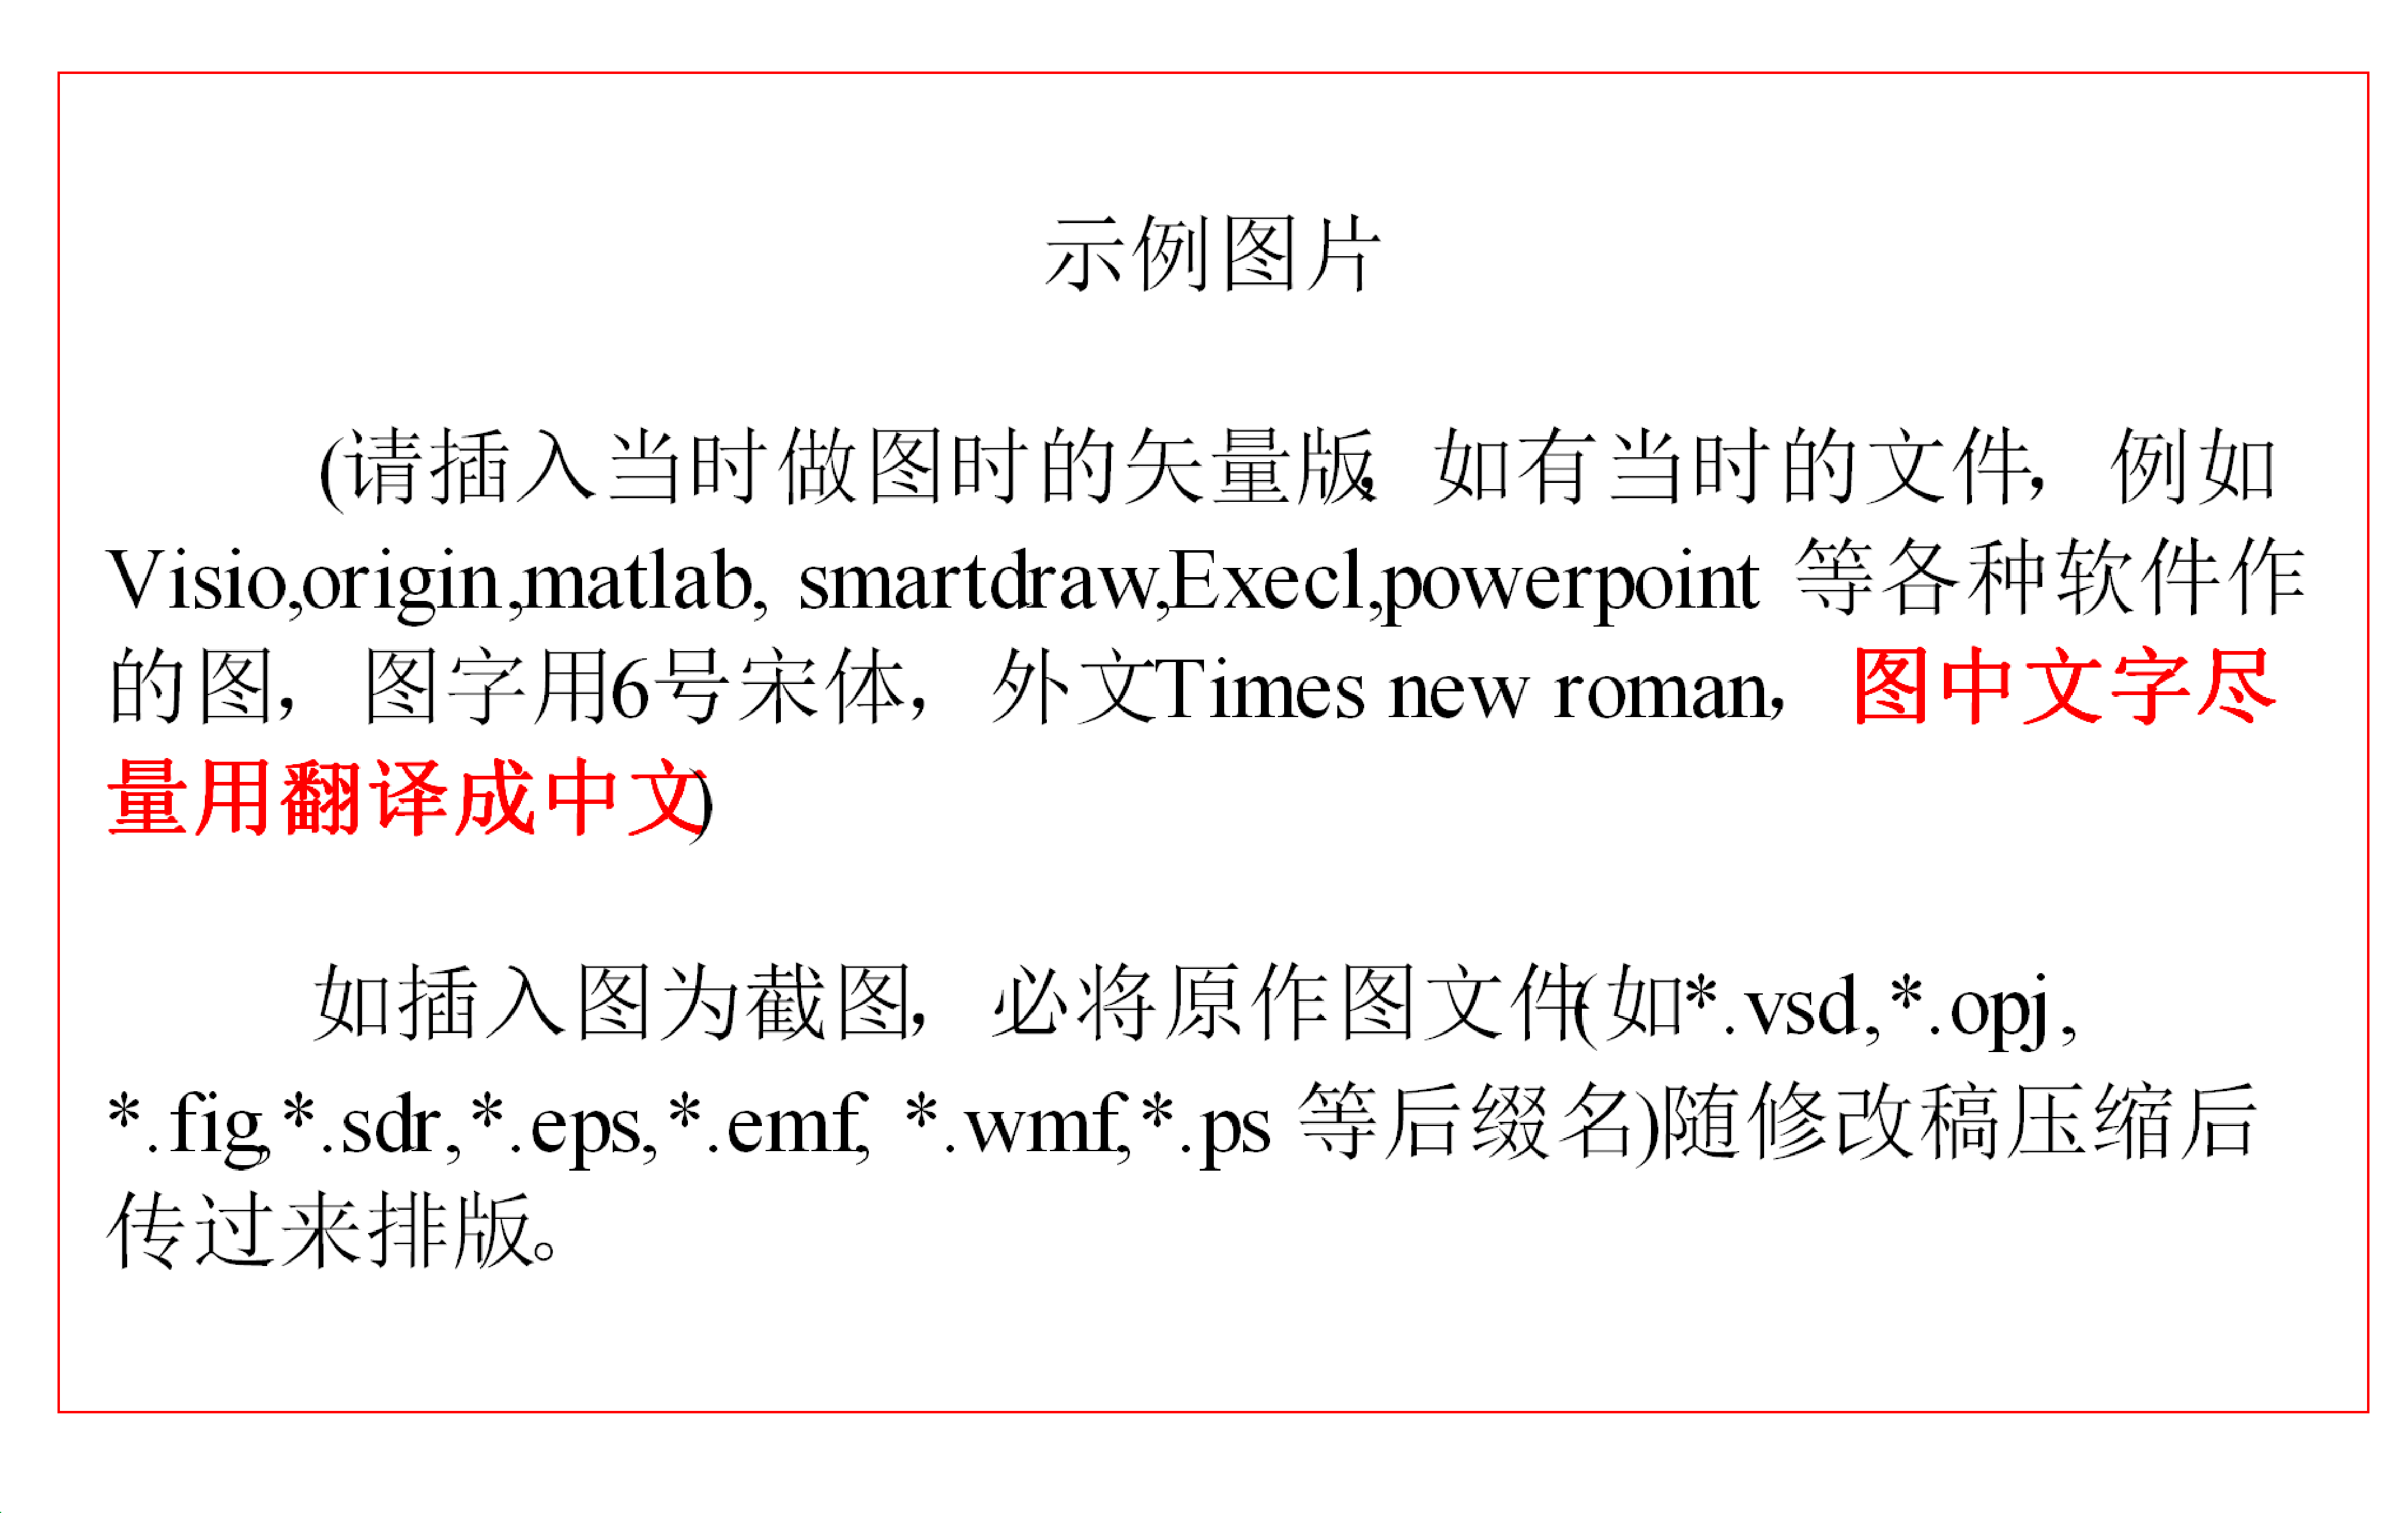
\includegraphics[width=3.15in,height=1.98in]{CJC1.pdf}}
图X\quad  图片说明 *字体为小5号,图片应为黑白图,图中的子图要有子图说明*
\label{fig1}
\end{figure}

\begin{table}[htbp]
\centering {\begin{CJK*}{UTF8}{zhhei}表X\quad 表说明 *表说明采用黑体*\end{CJK*}}
\vspace {-2.5mm}
\begin{center}
\begin{tabular}{ll}
\toprule
*示例表格*&*第1行为表头,表头要有内容* \\
\hline
&
 \\
&
 \\
&
 \\
&
 \\
\bottomrule
\end{tabular}
\label{tab1}
\end{center}
\end{table}

\begin{CJK*}{UTF8}{zhhei}过程X.\end{CJK*}\quad 过程名称

{\zihao{5-}*《计算机学报》的方法过程描述字体为小5号宋体,IF、THEN等伪代码关键词全部用大写字母,变量和函数名称用斜体*}


\begin{CJK*}{UTF8}{zhhei}算法\textbf{Y}\end{CJK*}.\quad 算法名称.
\zihao{5-}{

\noindent 输入:{\ldots} {\ldots}

\noindent 输出:{\ldots} {\ldots}

*《计算机学报》的算法描述字体为小5号宋体, IF、THEN等伪代码关键词全部用大写字母,变量和函数名称用斜体*}

\vspace {3mm}
\zihao{5}{
\noindent \begin{CJK*}{UTF8}{zhhei}致\quad 谢\end{CJK*}\quad \begin{CJK*}{UTF8}{kai} *致谢内容.* 致谢\end{CJK*}}


\vspace {5mm}
\centerline
{\zihao{5}
\begin{CJK*}{UTF8}{zhhei}参~考~文~献\end{CJK*}}

\begin{thebibliography}{99}
\zihao{5-} \addtolength{\itemsep}{-1em}
\vspace {1.5mm}

\bibitem[1]{ref1}
Sui Y, Zhou M, Zhou M, et al. Table meets llm: Can large language models understand structured table data? a benchmark and empirical study[C]//Proceedings of the 17th ACM International Conference on Web Search and Data Mining. 2024: 645-654.
  \end{thebibliography}

\begin{strip}
\end{strip}

\noindent {\zihao{5}\bf{附录X}.}

{\zihao{5-}\setlength\parindent{2em}
*\textbf{附录内容}置于此处,字体为小5号宋体。附录内容包括:\textbf{详细的定理证明、公式推导、原始数据}等*}

\begin{strip}
\end{strip}

\begin{biography}[yourphotofilename.jpg]
\noindent
\textbf{First A. Author}\ \ *计算机学报第1作者提供照片电子图片,尺寸为1寸。英文作者介绍内容包括:出生年,学位(或目前学历),职称,主要研究领域(\textbf{与中文作者介绍中的研究方向一致}).*
*字体为小5号Times New Roman*

\end{biography}

\begin{biography}[yourphotofilename.jpg]
\noindent
\textbf{Second B. Author} *英文作者介绍内容包括:出生年,学位(或目前学历),职称,主要研究领域(\textbf{与中文作者介绍中的研究方向一致})。*
*字体为小5号Times New Roman*
\end{biography}
\begin{strip}
\end{strip}
\zihao{5}
\noindent \textbf{Background}

\zihao{5-}{
\setlength\parindent{2em}
*论文背景介绍为\textbf{英文},字体为小5号Times New Roman体*

论文后面为400单词左右的英文背景介绍。介绍的内容包括:

本文研究的问题属于哪一个领域的什么问题。该类问题目前国际上解决到什么程度。

本文将问题解决到什么程度。

课题所属的项目。

项目的意义。

本研究群体以往在这个方向上的研究成果。

本文的成果是解决大课题中的哪一部分,如果涉及863$\backslash
$973以及其项目、基金、研究计划,注意这些项目的英文名称应书写正确。}

\end{CJK*}
\end{document}


